
\chapter{Rendering}

\begin{figure}
  \centering
    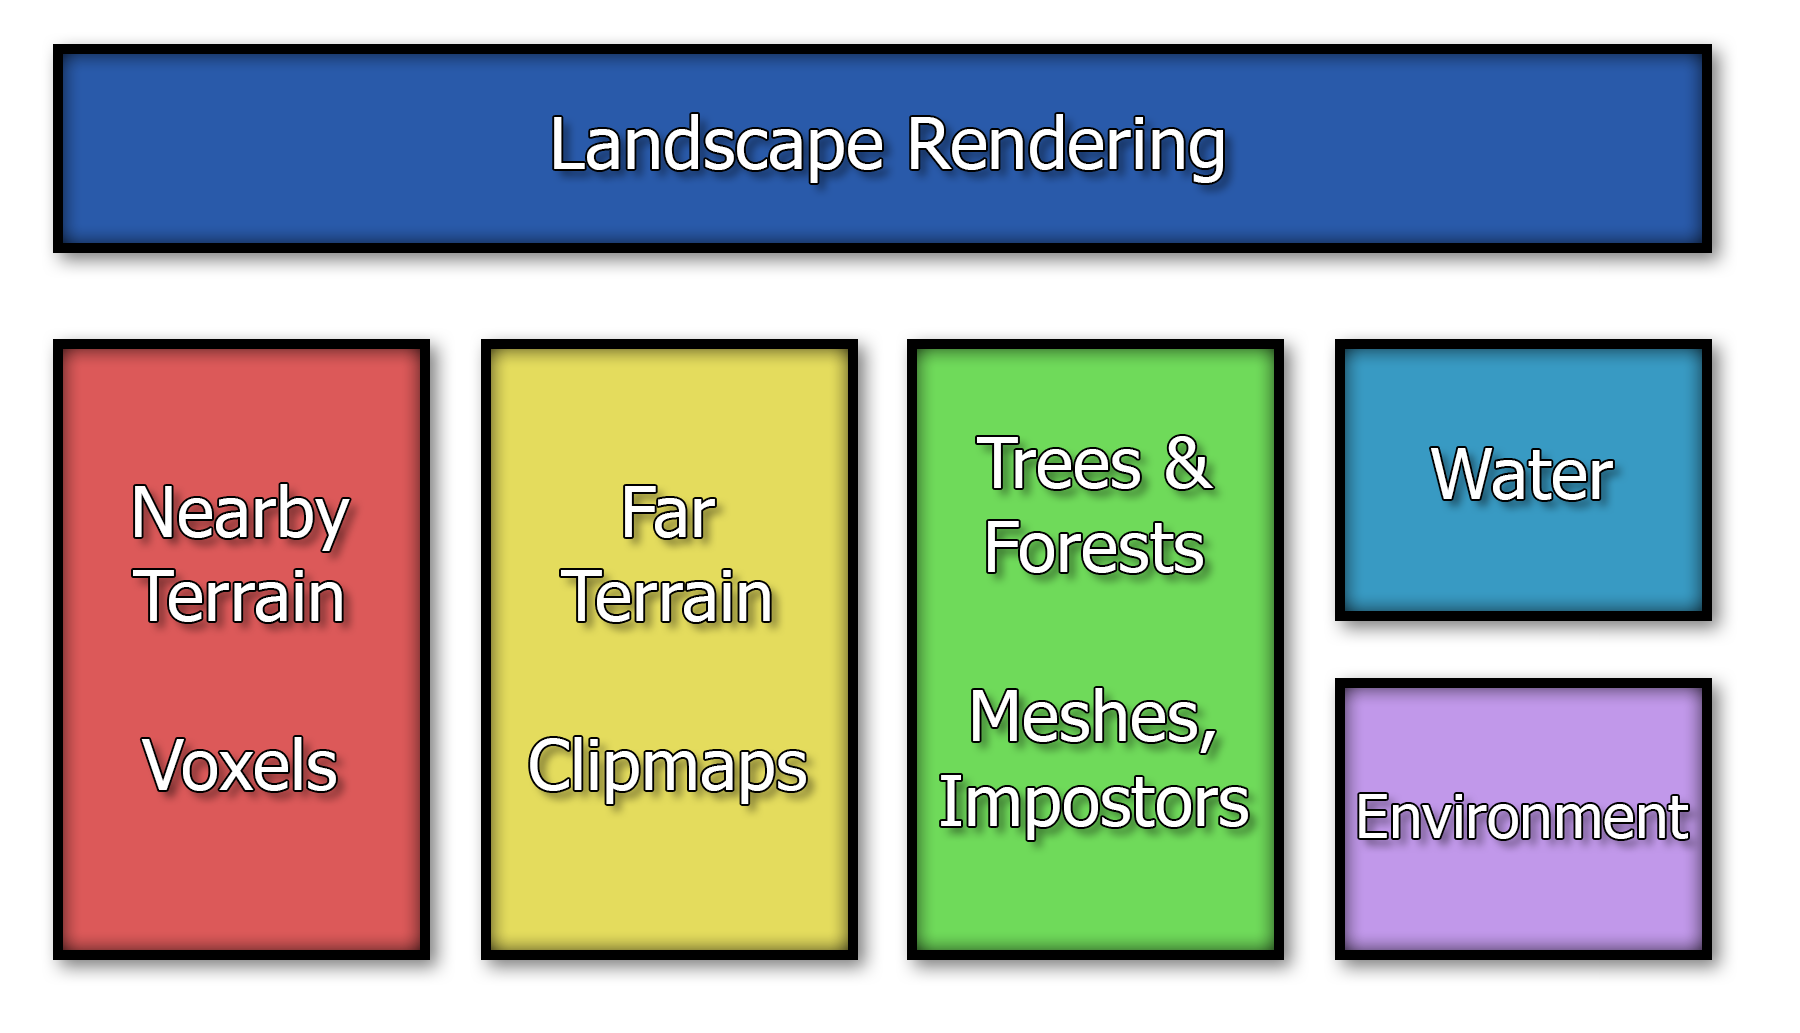
\includegraphics[width=0.8\textwidth]{figures/RenderSystem}
  \caption{Landscape rendering system overview}
  \label{fig:renderoverview}
\end{figure}

\editor{needs an into paragraph - what kind of rendering do you aim to support - what are the challenges given the setting - what are the basic technologies used to solve these problems (system diagram or bullet list).}

\section{Nearby Terrain} \label {voxterrain} %%%%%%%%%%%%%%%%%%%%%%%%%%%%%%%%%%%%%%%%%%%%%%%%%%%%%%%%%%%%%%%%%%%%%%%%%%%%%%%%%%%%%%%%%%%%%%%%%%%%%%%%%%%%%%%%%%%%%%%%%%%%%%%%%%%%%%

Nearby terrain is rendering using a pseudo-voxel representation designed to allow for sloped surfaces while maintaining intuitive live editing capabilities.
A voxel algorithm that uses uniform voxel size is simple to implement and manage but is poorly suited to represent sloped surfaces.
Fully volumetric terrain implementations allow for arbitrary slopes but are less intuitive for manipulation by players and navigation by AI.
We utilize a pseudo-voxel system that allows for diagonal faces in addition to solid voxels.
This system allows for simple grid-based editing and simple physics calculations, while allowing sloped polygonal faces that are more aesthetically pleasing than simple voxels.

\subsection{Voxel algorithm}

In principle, the system works by breaking down each individual voxel into 8 sub-voxels (one for each corner of the cube) and generating diagonal faces based on which of these sub-voxels are occupied.
However, certain sub-voxel configurations are considered degenerate and are automatically trimmed to a lesser configuration.
For example, in our system any pseudo-voxel with only a single sub-voxel occupied is automatically trimmed to an empty voxel.
In this case the trimming occurs because there is no diagonal face to represent just a single corner of a voxel.
Figure \editor{needed} shows the pseudo-voxel with the fewest possible sub-voxels, four.
The system can therefore trivially trim any pseudo-voxel configuration with fewer than four sub-voxels.

The system also trims certain pseudo-voxel configurations when the resulting triangle faces would simply confusing.
See Figure \editor{needed}.

\subsection{Face Generation}

Triangles are generated for each pseudo-voxel configuration using lookup tables for efficiency and simplicity.
Triangles are divided into two categories: interior and exterior.

\subsubsection{Exterior Faces}

Exterior triangles are the triangles that would normally be generated by a simple voxel system - the faces of a cube.
Exterior triangles are checked against each neighboring pseudo-voxel for visibility.
In the trivial case, a completely solid voxel surrounded entirely by solid voxels produces no triangles, since all exterior triangles are occluded by the exterior faces of each neighboring voxel.

Note that while a normal voxel system can arbitrarily decide how to triangulate the quad faces of a cube, our system must support either possible triangulation in order to match up with all possible diagonal faces.
See Figure \editor{needed} for an example of why arbitrary quad triangulation is needed.

\subsubsection{Interior faces}

Interior faces are what make the pseudo-voxel system interesting - any diagonal face that caps a partial pseudo-voxel.
See Figure \editor{needed} for a table of all interior faces.

\subsection{Rendering}

The world is divided into cube chunks for which a triangle mesh is generated.
Each chunk tracks its neighbors in all six face directions so that occluded exterior faces can always be accurately detected.
This means that a ring of non-visible chunks must be loaded around all visible chunks, since no visible chunk can have an unloaded neighbor.

Screen-space ambient occlusion is used to help visual understanding of the voxel terrain shape.


\section{Far Terrain} \label{clipterrain} %%%%%%%%%%%%%%%%%%%%%%%%%%%%%%%%%%%%%%%%%%%%%%%%%%%%%%%%%%%%%%%%%%%%%%%%%%%%%%%%%%%%%%%%%%%%%%%%%%%%%%%%%%%%%%%%%%%%%%%%%%%%%%%%%%%%%%%%%%%%%%%%%%%%%%%%%%%%%

Far terrain is rendered using a flat-shaded implementation of geometry clipmaps with a few modifications.

\subsection{Pre-calculated Index Buffer}

The original geometry clipmaps implementation recalculates index buffers pre-frame so that each layer can grow and expand organically.
This makes it possible to seamlessly transition to lower-resolution terrain when the viewpoint moves rapidly.

However, our system locks the size of each layer so that the index buffers can be pre-calculated.
This was found to significantly reduce CPU overhead

\subsection{Normal Calculation}

Since our terrain is flat-shaded for a polygonal effect, the per-quad normals provided by a normal map must be inaccurately applied to two triangles.
We also found that normal calculation from our procedural generation system incurred significant CPU overhead.
Accurate normal calculation in transition regions was also difficult.

Our implementation uses a per-triangle normal calculation in a geometry shader so that accurate normals are always calculated for each triangle.
This saves significant CPU time as normals don't need to be pre-calculated or sent to the GPU normal map.
The addition of the geometry shader was found to not have a significant decrease in rendering performance.


\section{Vegetation} %%%%%%%%%%%%%%%%%%%%%%%%%%%%%%%%%%%%%%%%%%%%%%%%%%%%%%%%%%%%%%%%%%%%%%%%%%%%%%%%%%%%%%%%%%%%%%%%%%%%%%%%%%%%%%%%%%%%%%%%%%%%%%%%%%%%%%%%%%%%%%%%%%%%%%%%%%%%%%

Our vegetation system currently supports rendering a large number of low-poly spruce trees, but could be expanded to support other types of vegetation.
The system uses three levels of detail: mesh instances, impostors, and mesh facades.

Trees are rendered in groups similar to the chunk system used by nearby terrain.
Mesh instances and impostors render many trees per group, whereas the mesh facade renders a single mesh to represent each group.

\subsection{Mesh Instances}

The mesh instances layer simply uses instance rendering to draw the tree model in several places.

\subsection{Impostors}

The impostors layer draws a billboard for each tree in the group.
During initialization, the colors and normals of the tree model are rendered to textures for use in drawing each impostor.
The impostors are locked in their X and Z axis rotation so that the base of the impostor always rests on the ground, and to reduce artifacts when the camera is high above or below the impostor.
See Figure \editor{need comparison of a tree billboard rotating around all axis}.
The rotation around the Y-axis is used to rotate the normals of the impostor so that lighting is accurate for impostors in all directions.

\subsection{Mesh Facades}

The final layer uses a simple mesh to represent a group of trees.
The appearance of this mesh is quite simplistic but at large view distances it is sufficient to represent a group of trees.
See Figure \editor{need close-up and distant view of a facade}.

\section{Water} %%%%%%%%%%%%%%%%%%%%%%%%%%%%%%%%%%%%%%%%%%%%%%%%%%%%%%%%%%%%%%%%%%%%%%%%%%%%%%%%%%%%%%%%%%%%%%%%%%%%%%%%%%%%%%%%%%%%%%%%%%%%%%%%%%%%%%%%%%%%%%%%%%%%%%%%%%%%%%%%%%%


Our water system uses the geometry of our far terrain (geometry clipmaps) implementation for simplicity.

Instead of offsetting each vertex by a heightmap value, however, we used summed Gerstner waves in the vertex shader.
This provides both a vertical offset and a normal to use for rendering.

The result is expensive, but simple and looks reasonable.


\section{Environment} %%%%%%%%%%%%%%%%%%%%%%%%%%%%%%%%%%%%%%%%%%%%%%%%%%%%%%%%%%%%%%%%%%%%%%%%%%%%%%%%%%%%%%%%%%%%%%%%%%%%%%%%%%%%%%%%%%%%%%%%%%%%%%%%%%%%%%%%%%%%%%%%%%%%%%%%%%%%%

The system renders a billboard to represent the sun and a sky sphere with vertex colors to represent the sky.

Lighting for all other objects in the scene uses three directional lights: one for direct sunlight, one for scene reflection of sunlight, and one for sky light.
The sunlight has high bright white color and points from the sun position towards the scene.
The scene reflection light has dim white color and points in the opposite direction of the sunlight, with the Y component clamped to zero.
The sky light points directly downward (negative Y) and has soft blue color.

Our system also implements a simple atmospheric scattering simulation by applying fog to each rendered fragment based on scene depth.
The fog color interpolates between dark blue for near fragments and the sky color for far fragments.
